% Grupo cociente G/H
% Compilar con: pdflatex quotient_group.tex
\documentclass[tikz,border=10pt]{standalone}
\usepackage{tikz}
\usepackage{amsmath}
\usepackage{xcolor}
\definecolor{gdlblue}{RGB}{41, 98, 168}
\definecolor{gdlred}{RGB}{191, 49, 49}
\definecolor{gdlgreen}{RGB}{30, 130, 76}
\definecolor{gdlorange}{RGB}{217, 130, 30}
\definecolor{gdlpurple}{RGB}{118, 56, 138}
\definecolor{gdlgray}{RGB}{140, 140, 140}
\definecolor{gdlyellow}{RGB}{190, 140, 10}
\usetikzlibrary{arrows.meta, positioning, patterns, calc}

\begin{document}
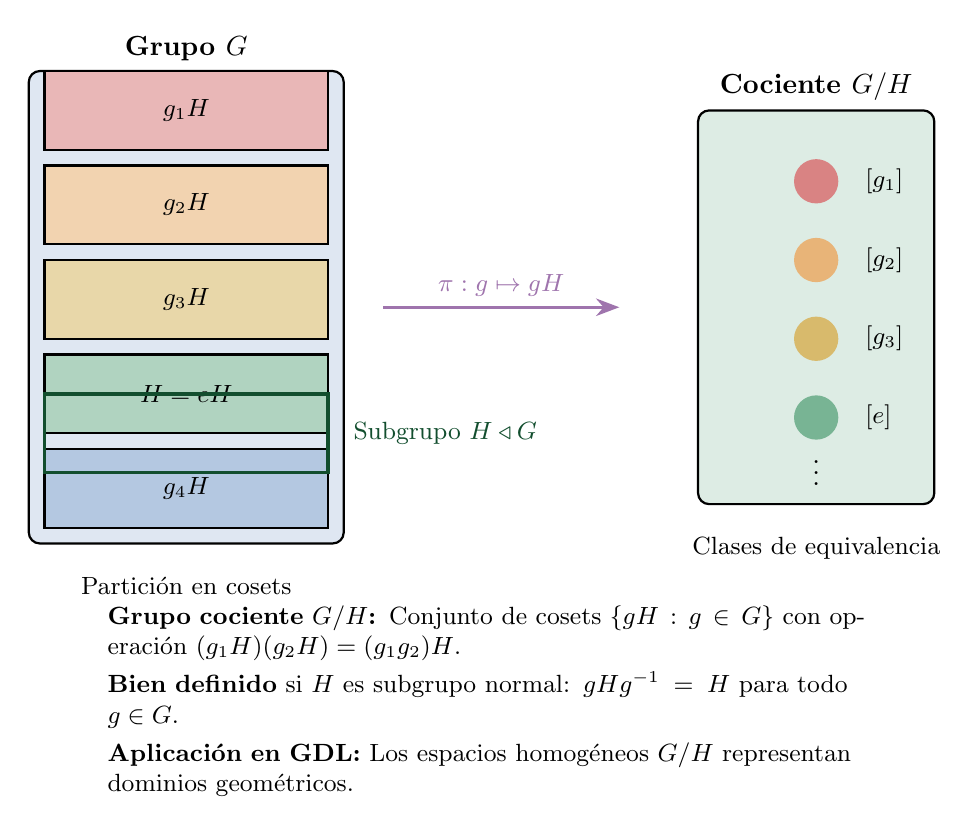
\begin{tikzpicture}[>=Stealth]

% === Grupo G ===
\begin{scope}[shift={(-4,0)}]
    \draw[thick, fill=gdlblue!15, rounded corners] (-2,-3) rectangle (2,3);
    \node[above, font=\bfseries] at (0, 3) {Grupo $G$};

    % Cosets de H (partición)
    \foreach \y/\col/\label in {
        2/gdlred!35/$g_1 H$,
        0.8/gdlorange!35/$g_2 H$,
        -0.4/gdlyellow!35/$g_3 H$,
        -1.6/gdlgreen!35/$H = eH$,
        -2.8/gdlblue!35/$g_4 H$
    } {
        \draw[thick, fill=\col] (-1.8, \y) rectangle (1.8, \y+1);
        \node[font=\small] at (0, \y+0.5) {\label};
    }

    % Etiqueta
    \node[below, font=\small] at (0, -3.3) {Partición en cosets};
\end{scope}

% === Flecha de proyección ===
\draw[->, very thick, gdlpurple!70] (-1.5, 0) -- node[above, font=\small] {$\pi: g \mapsto gH$} (1.5, 0);

% === Grupo cociente G/H ===
\begin{scope}[shift={(4,0)}]
    \draw[thick, fill=gdlgreen!15, rounded corners] (-1.5,-2.5) rectangle (1.5,2.5);
    \node[above, font=\bfseries] at (0, 2.5) {Cociente $G/H$};

    % Elementos del cociente (un punto por cada coset)
    \foreach \y/\col/\label in {
        1.6/gdlred!60/$[g_1]$,
        0.6/gdlorange!60/$[g_2]$,
        -0.4/gdlyellow!60/$[g_3]$,
        -1.4/gdlgreen!60/$[e]$
    } {
        \fill[\col] (0, \y) circle (8pt);
        \node[font=\small, right] at (0.5, \y) {\label};
    }

    % Puntos suspensivos
    \node at (0, -2) {$\vdots$};

    % Etiqueta
    \node[below, font=\small] at (0, -2.8) {Clases de equivalencia};
\end{scope}

% === Subgrupo H destacado ===
\begin{scope}[shift={(-4, -1.1)}]
    \draw[very thick, gdlgreen!60!black] (-1.8, 0) rectangle (1.8, -1);
    \node[gdlgreen!60!black, font=\small, right] at (2, -0.5) {Subgrupo $H \triangleleft G$};
\end{scope}

% === Leyenda ===
\node[font=\small, text width=10cm] at (0, -5) {
    \textbf{Grupo cociente $G/H$:} Conjunto de cosets $\{gH : g \in G\}$ con operación $(g_1 H)(g_2 H) = (g_1 g_2)H$.\\[0.3em]
    \textbf{Bien definido} si $H$ es subgrupo normal: $gHg^{-1} = H$ para todo $g \in G$.\\[0.3em]
    \textbf{Aplicación en GDL:} Los espacios homogéneos $G/H$ representan dominios geométricos.
};

\end{tikzpicture}
\end{document}
